\chapter{Étude numérique}
\label{Chap::Simu::Analysis}
	\minitoc

	Après avoir évoqué diverses propriétés des amas globulaires de notre galaxie puis étudié certains résultats
	analytiques concernant les propriétés dynamiques des systèmes auto-gravitant, nous allons maintenant mener des
	expériences numériques. Nous présenterons dans un premier temps le code d'évolution dynamique que nous avons
	utilisé, puis les conditions initiales de nos expériences et enfin les différentes observables de nos simulations.

	% \todo[inline]{FAIRE LA TRANSITION EN ANNONÇANT POURQUOI ON PASSE D'UNE DESCRIPTION FLUIDE À UNE PARTICULE À NOUVEAU.}

	% Après avoir mentionné l'importance des collisions à plusieurs corps pour expliquer le vieillissement des amas
	% d'étoiles, nous sommes passés dans la limite fluide afin de voir si d'autres phénomènes pouvait participer à
	% cette évolution. Nous allons maintenant nous tourner vers les simulations numériques.
	% Nous commencerons par présenter le treecode public Gadget-2. Nous enchaînerons sur la génération de nos
	% conditions initiales. Nous terminerons sur la présentation des diagnostiques nous servant à analyser les
	% simulations.

	% Après avoir montré l'importance des collisions à plusieurs corps dans les amas, puis être passé dans la
	% limite fluide afin de voir si d'autres phénomènes pouvait aussi faire évoluer ces amas. Nous nous retrouvons à
	% nouveau avec un système de particules que nous allons faire évoluer. Attention, il ne s'agit pas d'étoiles mais
	% de macro particules ayant une masse et une taille bien supérieur à celles des étoiles composant normalement ces
	% objets.

	% Les problèmes à $N$ corps sont des problèmes physiques extrêmement complexes mathématiquement: ils
	% font partie d'une famille d'équation du second ordre qui n'ont pas de solution pouvant
	% s'exprimer avec les fonctions mathématiques usuelles. Le seul cas connu pouvant s'écrire
	% simplement est le problème à 2 corps.

	\section{Le programme de simulation}
		% \todo[inline]{Parler macro-particule et limite fluide pour le $N$-corps.}

		Les expériences numériques que nous souhaitons réaliser ont pour objectif de modéliser l'évolution
		dynamique d'un système auto-gravitant. Dans ces simulations, nous souhaitons respecter au mieux le
		système du point de vue macroscopique (correspondant à la limite fluide de nos simulations).
		% tout en
		% laissant la possibilité à certains effets microscopiques d'apparaître (accrétion, relaxation).

		% Notre objectif est de résoudre numérique les équations de Vlasov-Poisson. Pour ceci, nous utilisons la
		% traditionnelle méthode $N$-corps: la fonction de distribution est échantillonée par des particules de
		% taille $\epsilon$, afin d'adoucir la force à petite échelle. En effet, nous souhaitons être au plus
		% proche de la limite fluide pour éviter les effets de relaxation à $N$-corps.

		% Le programme que nous utilisons pour faire évoluer notre système est
		Dans ce contexte, le programme que nous utilisons pour faire évoluer notre système est
		\textsc{Gadget-2}~\footnote{\url{http://www.mpa-garching.mpg.de/gadget/}} (voir \cite{gadget2} et \cite{gadget1}),
		écrit par Volker \textsc{Springel}.
		Ce programme allie un octree pour la gestion spatiale des particules et un algorithme de type \og
		prédicteur-correcteur\fg pour la partie temporelle.
		% Ce programme allie un octree pour calculer le potentiel avec un schéma d'intégration temporel de type \og prédicteur
		% correcteur\fg d'ordre 2 basé sur un \og leag-frog\fg.

		% En plus de permettre de faire des simulations cosmologiques, gadget implémente la physique nécessaire
		% pour faire des simulations de galaxie avec du gaz. Ou juste des simulations de systèmes de particules
		% sans effets autre que l'attraction gravitationnelle.

		% Ainsi, seule une petite partie de ce qu'il fait nous intéresse. En effet, nous n'allons utiliser que les options
		% concernant l'oct-tree. Toutes les autres options ne concernent que les simulations
		% cosmologiques ou pourraient induire un comportement non voulu du système ou du programme.
		% qui nous ferait perdre de la précision sur
		% les calculs.

		\subsection{Calcul du potentiel: $k^d$-Tree}
			\label{Sec::KdTree}
			% Numériquement, les problèmes à $N$-corps sont très couteux en terme de calculs. En effet, un
			% calcul simple de la force s'appliquant sur une particule peut se faire en sommant la force exercée par
			% chacune des autres particules dessus. Cette méthode nécessite une première itération sur toutes les
			% particules de la simulation, qui sera ensuite répétée pour toutes les particules. Elles
			% nécessitent donc $N^2$ opérations.
			% Ainsi, dés que nous allons tenter de simuler un grand nombre de particules, sur un grand nombre
			% de temps dynamique, les temps de calculs vont exploser.
			% Nous avons donc besoin d'un algorithme qui va nous permettre de faire évoluer le
			% système avec beaucoup de particule et sur un grand nombre de temps dynamique, dans des temps
			% raisonnables.

			Un calcul direct des forces d'interaction entre chaque particules nécessite $N^2$ opérations. Bien que très couteuse, cette
			méthode est encore très utilisée pour suivre finement la dynamique d'un amas. À ce jour, la plus grosse simulation $N$-corps
			directe est le travail de D. Heggie avec presque 300 000 particules (voir sa présentation au trimestre Gravasco) en utilisant
			la version GPU de NBODY6. Dans la limite fluide, nous aurons parfois besoin d'un grand nombre de particules pour représenter
			la fonction de distribution dans l'espace des phases. Nous avons donc besoin d'une approche nous permettant d'accélérer les
			calculs. Il existe de nombreuses méthodes le permettant. Celle que nous utilisons est basée sur un algorithme en arbre.

			% Un tel algorithme a été développé par J. Barnes et P. Hut dans~\citet{1986Natur.324..446B}. Il se
			% base sur un kd-tree de dimension 3, un oct-tree. Le principe est de subdiviser l'espace,
			% représenté par un cube, en 8 sous cubes, eux-mêmes subdivisé en 8 nouveaux sous cubes...
			% Chaque cube est à nouveau divisé s'il contient encore trop de particules.
			% Dans~\citet{1986Natur.324..446B}, ils arrêtent de subdiviser un cube quand il ne contient plus
			% qu'une particule; en pratique nous nous arrêterons lorsqu'un cube contiendra une quinzaine de
			% particules. La figure~\ref{Fig::KDTree::Repr} montre la structure d'un quad-tree, un
			% kd-tree à 2 dimension se construisant de la même façon.

			% Un tel algorithme a été appliqué en astrophysique pour la première fois par
			% \cite{1986Natur.324..446B}. Il se base sur une représentation en arbre
			% ($\mathrm{k}^\mathrm{d}$-Tree) des particules du système de dimension 3, cet arbre est appelé
			% octree ($k=2$, $d=3$). Le principe est de subdiviser un espace cubique en 8 sous cubes, eux-mêmes subdivisés en
			% 8 nouveaux sous cubes... Chaque cube est à nouveau divisé s'il contient encore trop de
			% particules.

			Cet algorithme, nommée \og treecode\fg, a été crée par~\cite{1986Natur.324..446B}.
			% Un tel algorithme a été appliqué en astrophysique pour la première fois par \cite{1986Natur.324..446B}.
			Les particules sont
			organisées dans un arbre modulable appelé $k^d$-Tree. En dimension $d=3$, et avec une division dichotomique
			($k=2$), cet arbre est un octree. Le principe est de subdiviser un espace cubique en 8 sous cubes, eux-mêmes subdivisés en 8
			nouveaux sous cubes... Chaque cube est à nouveau divisé s'il contient encore trop de particules.
			% Les auteurs arrêtent de diviser un cube quand il ne contient plus qu'une particule;
			En pratique nous nous arrêterons lorsqu'un cube contiendra au plus $N_\mathrm{max}=15$ particules. Les carrés et les points
			de la figure~\ref{Fig::KDTree::Parcours} montrent la structure d'un quadtree ($k=2$, $d=2$) se construisant de la même façon.
			% La figure~\ref{Fig::KDTree::Parcours} montre la structure d'un quadtree (un kd-tree à 2 dimension) se construisant de la
			% même façon.

			Avant de continuer il peut être utile de définir un peu de vocabulaire lié aux arbres:
			\begin{itemize}
				\item la racine constitue la base de l'arbre;
				\item un nœud est un cube ayant un père et des fils, il s'agit d'un embranchement;
				\item une feuille est un cube n'ayant plus de fils, et donc terminant une branche de
					l'arbre;
				\item une branche est le chemin à suivre pour aller de la racine vers une feuille.
			\end{itemize}

			% \begin{figure}
				% \begin{center}
					% 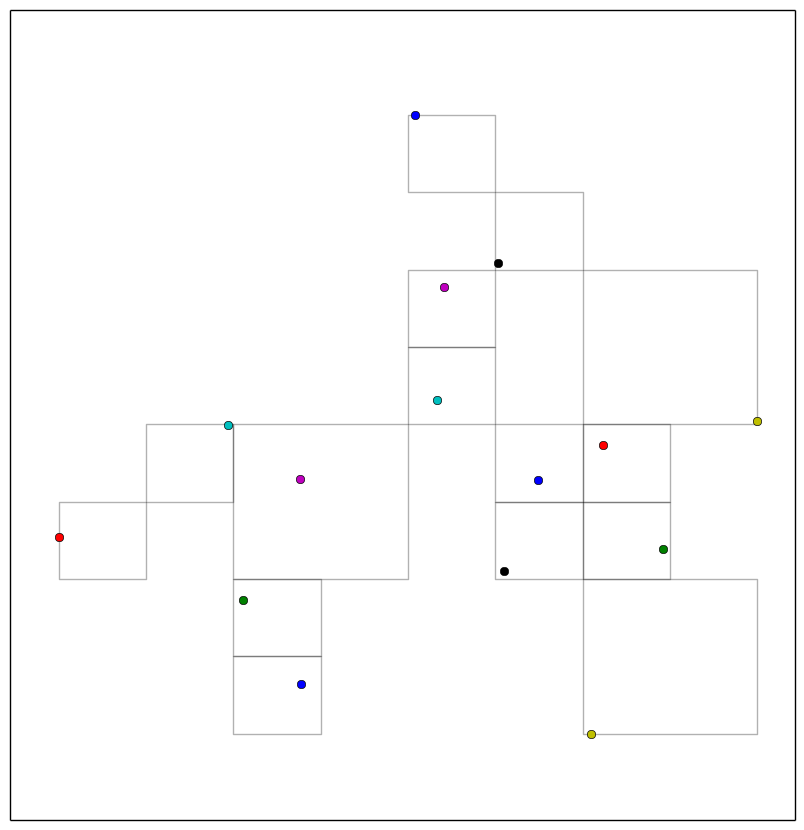
\includegraphics[scale=0.4]{repre_tree}
					% \caption{\label{Fig::KDTree::Repr}Représentation de la structure d'un quad-tree
						% (kd-tree en 2 dimension) sur 15 particules.}
				% \end{center}
			% \end{figure}

			Une fois l'arbre construit, le calcul de la force ou du potentiel se fait en descendant dans les nœuds
			tant que l'angle d'ouverture reste supérieur à une valeur critique.
			% (les cubes qui ont été subdivisés) selon un critère: l'angle d'ouverture du cube par rapport à une
			% particule est-il supérieur à une valeur $\theta$ choisie.
			L'angle d'ouverture correspond à la taille angulaire du nœud vue par la particule sélectionnée.
			Si cette taille est suffisamment petite, nous n'entrons pas à l'intérieur et résumons son
			contenu à une macro-particule, sinon la descente continue. Le critère d'ouverture est illustré par la
			figure~\ref{Fig::KDTree::Parcours}.
			% (voir figure~\ref{Fig::KDTree::Parcours})
			% nous testons chacune des
			% subdivisions. Par exemple, sur la figure~\ref{Fig::KDTree::Parcours}, le cône vert indique un
			% cube que nous ne voulons pas parcourir, tandis que le rouge nous indique qu'il faut continuer
			% à descendre.

			\begin{figure}
				\begin{center}
					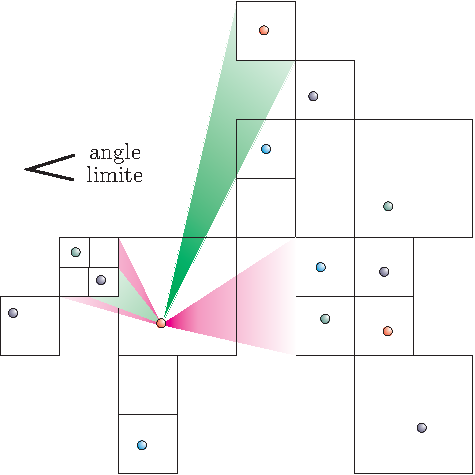
\includegraphics[scale=1.0]{accept_treev2}
					\caption{\label{Fig::KDTree::Parcours}
						Critère d'ouverture: le cône vert indique un carré qu'il n'est pas nécessaire d'ouvrir, le cône rouge
					indique un carré à ouvrir.}
						% Représentation du critère sur l'angle
						% d'ouverture pour ouvrir ou non un carré. Le cône vert indique un cube qu'il
						% n'est pas nécessaire d'ouvrir, le cône rouge indique un cube à ouvrir.}
				\end{center}
			\end{figure}

		\subsection{Lissage de la force}

			%Nous souhaitons nous placer dans la limite fluide afin
			%de minimiser les effets de relaxations dû aux
			%collisions à deux corps. Pour cela, nous pouvons jouer
			%sur deux paramètres : le nombre de particules que nous
			%mettons dans le système, et le paramètre de lissage.
			%Étant limité en temps, nous ne pouvons pas lancer de
			%simulations avec un très grand nombre de corps : les
			%plus grosses simulations que nous lançons ont 100 000
			%particules, et occasionnellement 500 000. Pour une
			%évolution pendant 100 temps dynamiques, elles prennent
			%environ 709 minutes en les faisant tourner sur 8 cœurs,
			%et cela peut aller jusqu'à 1020 minutes.

			%Toute la théorie a été faîte dans le cadre de l'équation de vlasov, et donc en supposant que nos
			%objet se comporte comme des fluides. Nous devons donc être sûr que les collisions interne de nos
			%objet n'aient que peu d'influence.
			%Pour éviter les soucis de divergence de la force lorsque deux
			%particules deviennent très proches, un paramètre de lissage (softening) a été introduite de façon à ce
			%que la force ne dépasse pas une valeur minimale. C'est aussi

			% Toute la théorie ayant été faite dans le cadre de la limite fluide, % l'équation de Vlasov,
			% nous souhaitons nous y placer aussi % dans la limite fluide
			% afin de nous approcher du mieux possible des conditions théoriques, mais
			% aussi pour minimiser les effets de relaxations à deux corps qui ne manqueront pas d'intervenir sur le long terme
			% dans cette description de nos système. Pour cela, nous allons jouer sur
			% le paramètre de lissage de la force qui adoucit cette dernière. Ceci ce traduit par le potentiel
			% effectif suivant:
			Toute la théorie ayant été faite dans le cadre de la limite fluide, % l'équation de Vlasov,
			il est important de l'approcher du mieux possible. %nous souhaitons nous y placer aussi % dans la limite fluide
			% afin de nous approcher du mieux possible des conditions théoriques, mais
			% Les effets de relaxations à deux corps sont également susceptibles d'intervenir sur le long
			% terme, il nous faut pouvoir les prendre en compte. % dans cette description de nos système.
			Pour cela, nous allons jouer sur
			le paramètre de lissage de la force $\epsilon$ dans le potentiel
			effectif suivant:
			% \todo[inline]{Je ne met pas la formule de Springel par ce que je ne la comprend pas vraiment. Il
			% utilise la convolution d'un dirac représentant la particule avec un "spline-kernel". Par
			% contre, pour la définition du $\epsilon$, c'est censé être équivalent à ceci.}
			% Classiquement, ce paramètre de lissage
			% est une borne, en distance, en deçà de laquelle nous considérons un potentiel minimum pouvant
			% s'écrire sous la forme:
			\begin{align}
				% \psi(r_{ij} \sim 0) = - G \dfrac{m_i}{r_{ij} + \epsilon}
				% \psi(r_{i}) = - G \sum_{j \neq i}^{N}\dfrac{m_i}{|r_{i}-r_j| + \epsilon}
				\psi(r_{i}) = - G \sum_{j \neq i}^{N}\dfrac{m_i}{r_{ij} + \epsilon}
			\end{align}
			où $r_{ij}$ est le module de distance entre les particules $i$ et $j$.
			Afin que la limite fluide soit suffisamment bien approché, nous devons choisir ce
			paramètre tel que d'une part la sphère de rayon $\epsilon$ contienne un nombre $N_\epsilon$ suffisant de particules
			mais que d'autre part $N_\epsilon$ soit suffisamment petit devant le nombre total de particules du système.
			Ce nombre $N_\epsilon$ peut s'évaluer de la façon suivante; considérons le paramètre
			\begin{align*}
				\alpha = \dfrac{\rho_\epsilon}{\rho_\mathrm{moy}}
			\end{align*}
			où $\rho_\epsilon$ la densité d'un volume de rayon $\epsilon$ suffisamment petit pour être
			supposé homogène et $\rho_\mathrm{moy}$ la densité
			moyenne de l'objet. Toutes les particules ayant la même masse, nous pouvons écrire:
			\begin{align}
				N_\epsilon    = \alpha N \(\dfrac{\epsilon}{R} \)^{3}
			\end{align}
			$N$ étant le nombre total de particules de l'amas. Les paramètres $N$, $R$ et $\alpha$ étant fixés, nous sommes
			ainsi libres de choisir $N_\epsilon$ ou $\epsilon$ pour répondre à nos besoins.

			Le code \textsc{Gadget-2} utilise une approximation plus sophistiquée consistant à approximer les particules par des nuages de
			taille $\epsilon$ et dont le profil suit une fonction \verb|spline|.

			% \begin{align}
				% \alpha = \dfrac{\rho_\epsilon}{\rho_\mathrm{moy}} = \dfrac{\rho_\epsilon}{M} \frac{4}{3} \pi R^3
			% \end{align}
			% où $M$ est la masse totale de l'amas, $R$ le rayon de l'amas, et $\rho(0)$ la densité centrale de
			% l'amas. La densité d'un volume de taille $\epsilon$ en fonction de la densité moyenne de l'amas
			% s'écrit alors:
			% \begin{align}
				% \rho_\epsilon &= \alpha \rho_\mathrm{moy}	\notag \\
				% \intertext{le nombre de particule dans un volume de rayon $\epsilon$ s'écrit:}
				% N_\epsilon    &= \alpha \frac{4}{3} \pi \epsilon^3 \dfrac{3N}{4\pi R^3}	\notag \\
					      % &= \alpha N \( \dfrac{\epsilon}{R} \)^{3}
			% \end{align}
			% $N$ étant le nombre total de particules de l'amas. $N$, $R$ et $\alpha$ étant fixés, nous sommes
			% ainsi libres de choisir $N_\epsilon$ ou $\epsilon$ pour répondre à nos besoins.

		\subsection{\og Leap-frog\fg et pas de temps}

			\textsc{Gadget-2} utilise un schéma d'intégration temporelle à pas de temps variable de type  \og prédicteur-correcteur\fg qui
			se ramène à un leap-frog, lorsque le pas de temps est constant, dont nous allons étudier le fonctionnement.

			Le prédicteur-correcteur utilisé est la combinaison suivante de deux opérateurs:
			\begin{align*}
				U(\Delta t) = K\(\frac{\Delta t}{2}\)D\(\Delta t\)K\(\frac{\Delta t}{2}\)
			\end{align*}
			où $\Delta t$ est le pas de temps d'une particule, $K$ l'opérateur permettant d'incrémenter la vitesse et $D$ la position.

			% Le problème simulé peut s'écrire ainsi:
			% Pour chaque particule de masse $m$ du système, le problème à résoudre s'écrit:
			% \begin{align*}
				% \begin{cases}
					% \dfrac{\vdr}{\dx{t}} = \vec{v} \\
					% \\
					% m\dfrac{\vdx{\vec{v}}}{\dx{t}} = \vec{f}(\vec{r})
				% \end{cases}
			% \end{align*}
			% il peut être approché par:
			% \begin{align*}
				% \begin{cases}
					% \dfrac{\vec{r}_\mathrm{new} - \vec{r}_\mathrm{old}}{\Delta t} = \vec{v}_\mathrm{new} \\
					% \\
					% m\dfrac{\vec{v}_\mathrm{new} - \vec{v}_\mathrm{old}}{\Delta t} = \vec{f}(\vec{r}_\mathrm{old}) = m\vec{a}
				% \end{cases}
			% \end{align*}
			La particularité du leap-frog est le décalage entre l'évaluation des positions est des vitesses:
			les positions vont être évaluées tous les $n\Delta t$ tandis que les vitesses vont l'être tout
			les $(n+\frac{1}{2})\Delta t$.
			Le schéma d'intégration s'écrit:
			\begin{align*}
				\begin{cases}
					\vec{v}_{n+1/2} = \vec{v}_{n-1/2} + \Delta t\vec{f}(\vec{r}_n) \\
					\\
					\vec{r}_{n+1} = \vec{r}_n +\Delta t\vec{v}_{n+1/2}
				\end{cases}
			\end{align*}

			Le code Gadget-2 opère une gestion fine du pas de temps $\Delta t$:
			\begin{align*}
				\Delta t = \sqrt{\dfrac{2\eta\epsilon}{|\vec{a}|}}
			\end{align*}
			de manière à ce qu'il reste dans un intervalle de contrôle.
			Le paramètre $\eta$ permet de contrôler la précision de l'intégration, $\vec{a}$ est l'accélération.

			L'intérêt de ce schéma d'intégration est qu'il assure une excellente gestion de l'énergie du système; ce type d'intégrateur est dit symplectique.

			% Il reste à déterminer comment le pas de temps $\Delta t$ est calculé dans Gadget-2. La première chose à
			% laquelle faire attention est que chaque particules a son propre pas de temps. Ce pas de temps
			% va évoluer au cours de la simulation, tout en restant bornée par un pas de temps minimum et un
			% pas de temps maximum. Le pas de temps est donné par la formule:
			% \begin{align*}
				% \Delta t = \sqrt{\dfrac{2\eta\epsilon}{|\vec{a}|}}
			% \end{align*}
			% où $\epsilon$ est le paramètre de lissage de la force, $|\vec{a}|$ le module de l'accélération
			% de la particule et $\eta$ un paramètre permettant de contrôler la précision de l'intégration.

		%\subsection{Unités}

			%Dans ce fichier, nous n'allons jouer que sur certains paramètres :
			%\begin{itemize}
				%\item \verb|OmegaLambda| : paramètre cosmologique représentant la densité d'énergie du
					%vide, en le mettant à 0, nous faisons savoir à \textsc{Gadget-2} que nous ne faisons pas
					%de simulation cosmologique.
				%\item \verb|UnitLength_in_cm|, \verb|UnitMass_in_g| et \verb|UnitVelocity_in_cm_per_s|
					%sont les unités dans lesquelles sont données, respectivement, les positions, masses et vitesses des particules en
					%centimètre, gramme en centimètre par seconde. Ce sont ces facteurs de conversion
					%qui donne l'unité de temps interne à \textsc{Gadget-2}. Nous utilisons
					%les parsecs ($ 1 pc = 3.086 \times 10^{18} cm$) pour les positions, les kilogrammes
					%($1 kg = 1000 g$) pour la masse, et les mètres par seconde ($ 1 m.s^{-1} = 10^2 cm.s^{-1}$)
					%pour les vitesses. Ces unités nous donnent comme unité de temps
					%interne :
					%\begin{align}
						%v &= \frac{d}{t} \notag \\
						%t &= \frac{d}{v} \notag \\
						%t &= \frac{3.086 \times 10^{18}}{10^2} = 3.086 \times 10^{16} s \notag \\
						%t &= 9.77894 \times 10^8 ans
					%\end{align}
				%\item \verb|SofteningStarsMaxPhys| : paramètre de lissage de la force, permettant d'éviter
					%qu'elle \og~n'explose~\fg~à cause d'une collision entre 2 particules trop proches.
					%C'est sur ce paramètre qu'il faut jouer pour assurer la stabilité du système sur
					%un grand nombre de temps dynamiques.
				%\item \verb|ErrTolTheta| : représente l'angle d'ouverture, ou résolution angulaire, minimum.
					%Celui-ci est fixé à $0.5$ et n'est plus modifié ensuite.
			%\end{itemize}






		%Pour fonctionner, \textsc{Gadget-2} a besoin d'un fichier de
		%configuration, dans lequel nous devrons jouer sur certains
		%paramètres, et d'un fichier de conditions initiales respectant
		%un format précis.

		%\subsection{Pas de temps}
		%\subsection{Paramètre de l'arbre}
		%\subsection{Format de sortie}

		%\subsection{Fichier de conditions initiales}

			%Le fichier de conditions initiales doit avoir le format suivant :
			%\begin{enumerate}
				%\item un en-tête contenant le nombre de particule de chaque type (~Gaz, Halo, Disque, Bulbe, Étoiles, Bndry~),
				%la masse pour chaque type, divers autres informations utiles essentiellement aux simulations cosmologiques,
				%\item les positions de chaque particules,
				%\item leurs vitesses,
				%\item un identifiant permettant de repérer chaque particule.
			%\end{enumerate}
			%Chaque bloc devant être encadré par sa taille en mémoire.

		%\subsection{Fichier de configuration}



	\section{Conditions initiales}

		% Pour générer des nombres aléatoires dans l'intervalle voulu, nous utiliserons une
		% implémentation de la fonction \verb|ran2| tiré de~\citet{NumericalRecipesC}.

		Pour mener à bien nos expériences numériques, nous avons besoin de plusieurs configurations: une sphère de King,
		une sphère de Hénon et un bain thermique.

		\subsection{Le modèle de \textsc{King}}

			Les particules du modèle de King, de paramètres $W_0$, $\sigma$ et $r_c$ sont générées en
			utilisant une méthode d'acceptation-rejection que nous allons décrire. À partir de ces 3
			paramètres, nous pouvons résoudre l'équation de poisson~(\ref{King-Pois}) donnant le potentiel
			pour le modèle de King. Nous pouvons alors calculer le potentiel central $\psi(0)$ et l'énergie
			de libération $E_l$.
			% Ces particules sont telles que $r<R$ et $v<v_\mathrm{max}$, avec $R$ et $v_\mathrm{max}$ défini tels que:
			Toutes les particules de la sphère de King ont une vitesse dont le module de vitesse est
			inférieur à une vitesse $v_\mathrm{max}$ et leurs distance au centre est inférieur à un rayon
			$R$. Ces bornes sont définies tel que:
			% Pour obtenir nos conditions initiales, qui devront suivre un profil de \textsc{King}, nous
			% allons utiliser la méthode de réjection. Nous allons tirer aléatoirement la position et la
			% vitesse des particules dans une boîte, puis nous n'en garderons qu'une partie en utilisant la
			% fonction de distribution dans l'espace des phases comme une densité de probabilité. Pour
			% commencer, nous utilisons les limites du modèle pour restreindre nos tirages à une boîte de
			% taille \mbox{$\left[ - R; R \right]$} pour les distances et \mbox{$\left[ -v_{\mathrm{max}};
			% v_{\mathrm{max}}\right]$} pour les vitesses, avec:
			% \begin{itemize}
				% \item $v_{\mathrm{max}}$ la vitesse maximum: %l'énergie totale du système est bornée supérieurement par l'énergie de libération :
			la vitesse maximale $v_{\mathrm{max}}$ est donnée par la relation:
					\begin{align}
						% E = \dfrac{1}{2} m v_i^2 + m\psi(r) &< E_l \notag \\
						% E_l - m\psi(r) &> \dfrac{1}{2} m v_i^2 \notag \\
						% v_\mathrm{max}^2 = 2\(\dfrac{E_l}{m} - \psi(r)\) &> v_i^2 \notag \\
						v_{\mathrm{max}} = \sqrt{2\(\dfrac{E_l}{m} - \psi(0)\)}% > v_i &> - \sqrt{2\(\dfrac{E_l}{m} - \psi(0)\)} = - v_{\mathrm{max}}
					\end{align}
				% \item $R$
					le rayon $R$ de la sphère est obtenu en résolvant numériquement
				% \item $R$ la distance maximum : cette distance est obtenue pour
					% $m\psi(R) = E_l$.
					$\rho(R) = 0$.
			% \end{itemize}
			% où $E_l$, l'énergie de libération est déterminé, grâce au théorème de Gauss, par:
			% \begin{align*}
				% \dfrac{E_l}{m} = -\dfrac{GM}{R}
			% \end{align*}

			Les paramètres $R$ et $v_\mathrm{max}$ étant connus, nous tirons aléatoirement les positions
			$x_i$, $y_i$, $z_i$ telles que $|\vec{r}_i| \leq R$; puis les vitesses $v^x_i$, $v^y_i$, $v^z_i$
			telles que $|\vec{v}_i|\leq v_\mathrm{max}$.
			% Formule obtenue en considérant que l'énergie qu'une particule de vitesse nulle au centre du
			% système doit acquérir est donnée par l'énergie su
			% Il nous faut donc connaître le potentiel, qui est obtenu numériquement.

			%Le potentiel n'ayant pas d'expression analytique, nous
			%allons devoir réutiliser notre algorithme de résolution numérique utilisé dans les chapitres
			%précédents pour modèliser un King.

			%Il nous faut aussi pouvoir redimensionner les quantités obtenues. Pour cela, le
			%programme récupère dans un fichier de configuration les dispersions de vitesse
			%$\sigma_v^2$, rayon de c\oe ur $r_c$, temps de relaxation $T_c$ et distance au
			%soleil $R_\odot$ dans les unités du catalogue de \textsc{Harris}. Toutes sont
			%ensuite transformées en unités SI (~mètre, kilogramme, seconde~). Comme nous
			%avons pu le voir dans le chapitre~\ref{King::Chapitre} traitant du modèle de
			%King, la masse $m$ d'une particule n'influence pas le profil de densité final :

			% Les simulations utilisant le modèle de \textsc{King} s'effectueront en unités physique,
			% En connaissant le rayon de cœur $r_c$ et la dispersion de vitesse $\sigma_v$, il est possible de
			% déduire la dernière quantité nécessaire au dimensionnement: $\rho_0$ (défini dans le
			% chapitre~\ref{King::Chapitre}). Reste ensuite une degré de
			% liberté qui nous permet de choisir entre la masse d'une particule ou le nombre de
			% particules du système.
			% \begin{align}
				% r_c^2 &= \dfrac{\sigma^2}{4\pi G m \rho_0} \notag \\
				      % &= \dfrac{(\sigma_v^2)^2 m}{8\pi G m \rho_0} \notag \\
				      % % &= \dfrac{(\sigma_v^2)^2}{8\pi G \rho_0} \notag \\
				% \Rightarrow \rho_0 &= \dfrac{(\sigma_v^2)^2}{8\pi G r_c^2}
			% \end{align}
			% Pour redimensionner la densité, nous n'avons donc pas besoin de connaître la
			% masse d'une particule. Ce constat nous permet de laisser ce paramètre libre et
			% de jouer sur le nombre de particules dans le système. En effet, une fois la
			% densité obtenue, nous pouvons l'intégrer sur le volume de l'amas pour trouver la
			% masse totale de ce dernier, puis, connaissant le nombre de particules, en déduire
			% la masse d'une étoile par la relation :
			% \begin{align}
				% m = \dfrac{M_{tot}}{\text{Nombre de particules}}
			% \end{align}
			% Déduire le reste des paramètres utiles pour le redimensionnement est ensuite
			% assez simple.
			% La distance maximum $r_{\mathrm{max}}$ est déduite de la résolution
			% numérique des équations.

			% Pour pouvoir tout redimensionner, nous avons aussi besoin de connaître l'énergie
			% de libération de l'amas $E_l$. Pour cela, nous utilisons le théorème de \textsc{Gauss}.
			%et un petit raisonnement simple.
			% Par définition, nous avons :
			% \todo[inline]{Reformuler cette partie sur les énergies, je ne pense pas transmettre la bonne
			% idée.}
			% \begin{align}
				% E_\mathrm{min} < E < E_l < 0 \ &\text{ et } \ E_l = \frac{p^2}{2 m} + m \psi(r)
				% \intertext{soit:}
				% \intertext{le maximum du potentiel est atteint lorsque $p=0$, en appliquant le théorème
				% de Gauss au bord du système:}
				% \psi(r) = \frac{1}{m}\(E_l - \frac{p^2}{2 m}\)
				% \intertext{La valeur maximale du potentiel est donc atteinte pour $p = 0$ :}
				% \psi_\mathrm{max} = \psi(R) = \frac{E_l}{m} \stackrel{\mathrm{Gauss}}{=} -\frac{G M}{R}
				% \intertext{Hors du système, le théorème de \textsc{Gauss} nous dit qu'il peut être vu comme une particule ponctuelle de masse $M$. Le potentiel hors de l'amas s'écrit donc :}
				% \psi(r) = -\frac{G M}{r}
				% \intertext{Par continuité, nous avons :}
				% \psi(R) = \frac{E_l}{m} = -\frac{G M}{R}
			% \end{align}

			% Pour générer des nombres aléatoires dans l'intervalle voulu, nous utilisons la
			% fonction \verb|double ran2(long seed)| tiré de~\citet{NumericalRecipesC}, dont
			% nous nous servont ainsi :
			% \lstset{language=C, label=algo::tirage, frame=shadowbox}
			% \begin{lstlisting}
				% double  x  = rmax - 2.0 * rmax * ran2(seed),
					% y  = rmax - 2.0 * rmax * ran2(seed),
					% z  = rmax - 2.0 * rmax * ran2(seed),
					% vx = vmax - 2.0 * vmax * ran2(seed),
					% vy = vmax - 2.0 * vmax * ran2(seed),
					% vz = vmax - 2.0 * vmax * ran2(seed);
			% \end{lstlisting}

			% Jusqu'ici, nous avons généré nos particules dans un cube. L'étape suivante consiste à les
			% filtrer selon leur distance au centre.
			% L'étape suivante consiste à les filtrer en utilisant la fonction de distribution dans l'espace
			% des phases comme une densité de probabilité.
			% Pour le modèle de King, nous connaissons $f(E)$ et non $f(\vec{r}, \vec{v})$; nous calculons
			% donc l'énergie à partir des positions et vitesses.

			Nous utilisons alors la fonction de distribution du modèle de King (voir la
			relation~\ref{King::Eq::DistribFunc}) normalisée à $1$ comme une densité de probabilité, en
			utilisant l'énergie $E_i = \frac{1}{2}mv_i^2 + m\psi(r_i)$, pour accepter ou rejeter la
			particule $i$ fabriquée. Le taux de rejection est de l'ordre de $99.99\%$
			mais la vitesse des ordinateurs permet d'utiliser cette méthode très simple pour fabriquer un
			modèle de King discret.
			% mais cette méthode permet de générer simplement un modèle de King.

			% À la fin, nous regardons la probabilité d'avoir une
			% particule avec ces valeurs de positions et vitesses et nous tirons un nombre aléatoire nous
			% disant si la particule est conservée ou non.


			% Notre système étant sphérique, nous ne devons pas avoir
			% de vitesse et de module de distance supérieurs,
			% respectivement, à $v_{\mathrm{max}}$ et
			% $r_{\mathrm{max}}$, de plus nous avons une probabilité
			% \mbox{$f(E)/f(E_\mathrm{min})$} d'avoir une particule
			% d'énergie $E$. Cette énergie minimale est l'énergie
			% potentielle d'une particule au centre de l'amas, et de
			% vitesse nulle. Une fois qu'une particule respecte ces
			% conditions et que \og les probabilités sont avec
			% elle\fg, nous l'enregistrons.

			% Le programme écrit au fur et à mesure les coordonnées cartésiennes et vitesses
			% des particules sélectionnées dans un fichier dans les unités standards : mètre
			% pour les distances et mètre par seconde pour les vitesses.

		\subsection{La sphère de Hénon}

			% Une sphère de Hénon est, comme son nom l'indique, une sphère de densité
			La sphère de Hénon (\cite{1964AnAp...27...83H}) est une sphère de densité
			constante $\rho_0$ possédant une distribution de vitesse suivant
			une loi de Gauss:
			\begin{align}
				f_H(r, v) = \rho_0 e^{-v^2/\sigma^2}
			\end{align}
			Nous générons donc indépendamment les positions selon une loi uniforme, et les vitesses selon
			une loi gaussienne. Le choix de la dispersion de vitesse $\sigma$ nous permet de choisir le rapport
			du Viriel $\gamma = \dfrac{2E_c}{E_p}$ de la sphère à l'instant initial.
			% La dernière étape consiste à modifier les vitesses pour mettre le système au
			% Viriel $\gamma = -\dfrac{2E_c}{E_p}$ voulu.

		\subsection{Bain thermique}

			Lors de notre étude numérique, nous allons avoir besoin de créer un objet nous permettant de
			simuler un bain thermique. Pour ceci, nous allons utiliser un cube homogène de côté $R_c$
			possédant un distribution de vitesse gaussienne de dispersion $\sigma_c$.
			Nous jouerons sur ces deux paramètres pour tester l'influence du bain.

	\section{Observables des simulations}  %\label{Verif_gene}}

		% Maintenant que nous avons un générateur de conditions
		% initiales, il convient de le vérifier. C'est-à-dire d'utiliser
		% les coordonnées, vitesses et masses des particules pour
		% remonter à des quantités comme la densité ou l'énergie de
		% l'objet créé, puis de comparer ces quantités aux prédictions
		% théoriques. À des fins de Comparaison, nous avons généré un
		% profil de King avec \mbox{100 000} particules, qui se doit donc d'être
		% au Viriel, mais aussi d'avoir un profil de densité de type cœur-halo.

		Lors de nos expériences numériques, nous souhaitons étudier l'évolution des paramètres des systèmes. Nous avons donc construit un code
		effectuant le calcul de différentes observables spatiales (densité, position, rapport d'axes, etc) et cinétiques (énergies,
		température, etc).

		Toutes les courbes présentées dans cette section correspondent à un modèle de King de paramètre $W_0=6$, $r_c =
		3.5\mathrm{pc}$ et $\sigma_v = 2.9 \mathrm{km}.\mathrm{s}^{-1}$ généré avec 100 000 particules.

		% Nous en profiterons pour présenter toutes les quantités diagnostiqué.
		% densité, comme vu dans les précédents chapitres.

		% Pour faire les vérifications, nous avons choisi d'utiliser des histogrammes.

		\subsection{Recentrage}

			Pour calculer avec précision les différentes quantités physiques qui nous intéressent, il est
			important d'avoir la meilleure détermination possible du centre du système, qui a tendance à se
			déplacer. Ce déplacement peut se produire car la vitesse moyenne du système n'est pas exactement
			nulle, ou encore parce que des particules sont éjectées loin du système, emportant une partie
			notable de l'énergie.

			% Lors des simulations, nos systèmes peuvent se déplacer. Par exemple, un système isolé va voir sa
			% vitesse moyenne augmentée en perdant des particules. Ou encore parce que la vitesse moyenne du
			% système à $t=0$ n'est pas exactement nulle.

			Plusieurs méthodes sont envisageables pour recentrer le système. La première est de calculer le
			centre de gravité. Le problème posé par cette approche est que les particules très éloignées du
			centre système ont le même poids statistique que les particules proches du centre.
			Le calcul du centre de gravité peut s'en trouver largement affecté.
			Par conséquent, nous devons calculer un centre en donnant plus de poids aux
			particules se trouvant dans des zones denses du système. Il s'agit du \og centre de densité\fg,
			tel que décrit dans~\citet{1985ApJ...298...80C}. Le principe est de rechercher les $j$ plus
			proches voisins d'une particule et de regarder dans quel volume elles se répartissent; ceci nous
			donne la densité locale de la particule, et donc son poids selon la formule suivante:
			\begin{align}
				\rho_j^i = \dfrac{j-1}{V(r_j)}m
			\end{align}
			avec $j$ le nombre de voisin, $\rho_j^i$ la densité locale à la particule $i$, $V(r_j)$ le volume
			dans lequel se situent les $j$ voisins, et $m$ la masse d'une particule. Pour obtenir le centre
			de densité,
			nous faisons un calcul similaire au centre de gravité mais en pondérant chaque position par sa densité locale.

			Ce calcul peut s'avérer numériquement couteux, nous avons  donc adapté l'algorithme de l'octree
			pour accélérer le calcul.
			% Pour accélérer les calculs, nous utilisons la technique de l'octree décrite précédemment afin de chercher les $j$ plus
			% proches voisins, mais plutôt que d'utiliser l'angle d'ouverture, nous comparons
			% la distance entre la particule $i$ et le coin le plus proche de chaque cube à la distance entre
			% la particule $i$ et le voisin trouvé le plus lointain. Si le cube est plus proche, il est alors
			% sélectionné et nous testons ses fils ou les particules si nous sommes sur une feuille.

		\subsection{Masse et densité}

			\begin{wrapfigure}{l}{0.40\textwidth}
				\begin{center}
					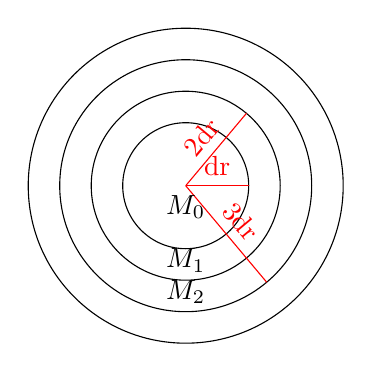
\begin{tikzpicture}[scale=0.8]
						\draw (2.5,2.5) circle(1);
						\draw (2.5,2.5) circle(1.5);
						\draw (2.5,2.5) circle(2);
						\draw (2.5,2.5) circle(2.5);
						\draw[red] (2.5,2.5) -- (3.5,2.5) node[midway, above] {$\mathrm{dr}$};
						\draw[red] (2.5,2.5) -- ++(50:1.5) node[sloped, above, midway] {$2 \mathrm{dr}$};
						\draw[red] (2.5,2.5) -- ++(-50:2) node[sloped, above, midway] {$3 \mathrm{dr}$};
						\draw (2.5,2.5) node[below]{$M_0$};
						\draw (2.5,1.15) node[below]{$M_2$};
						\draw (2.5,1.65) node[below]{$M_1$};
					\end{tikzpicture}
				\end{center}
				\caption{Découpage de l'amas généré pour des coquilles espacées linéairement.\label{schema::bin}}
			\end{wrapfigure}
			Le premier histogramme que nous générerons sera celui
			représentant la masse en fonction du rayon. Notre objet
			étant sphérique, nous allons le découper en coquilles d'épaisseur
			$\mathrm{dr}_i$ variable.
			% La fonction de masse représente la masse se trouvant
			% dans l'intervalle \mbox{$\left[0; j
			% \mathrm{dr}\right]$}.
			Pour la calculer, nous comptons
			le nombre de particules dans chaque chaque coquille
			sphérique de largeur $\mathrm{dr}$, puis, après avoir
			multiplié par la masse d'un particule, nous sommons,
			pour le bin $j$, tous les bins inférieurs.

			En même temps que nous calculons la fonction de masse, nous pouvons calculer la
			densité en divisant la masse dans un bin par le volume du bin :
			\begin{align}
				\rho_\mathrm{bin} &= \dfrac{M_\mathrm{bin}}{V_\mathrm{bin}} \notag \\
				\rho(r_i + \mathrm{dr}_i) &= \dfrac{M(r_i + \mathrm{dr}_i) - M(r_i)}{V(r_i + \mathrm{dr}_i) - V(r_i)}
				% \rho_i = \rho\( (i+1) \mathrm{dr}\) &= \dfrac{M_{\mathrm{bin}\ i}}{V_{\mathrm{bin}\ i}} = \dfrac{3 \(M_i - M_{i-1}\)}{4 \pi \mathrm{dr}^3 \left[ 3 i^2 + 3 i + 1\right]}
					% &= \dfrac{M_{\mathrm{bin}\ i}}{\frac{4}{3}\pi ( (i+1)\mathrm{dr})^3 - \frac{4}{3}\pi ( i\mathrm{dr})^3} \notag \\
					% &= \dfrac{3 M_{\mathrm{bin}\ i}}{4 \pi \mathrm{dr}^3 \left[ (i+1)^3 - i^3\right]} \notag \\
					% &= \dfrac{3 M_{\mathrm{bin}\ i}}{4 \pi \mathrm{dr}^3 \left[ 3 i^2 + 3 i + 1\right]} \notag \\
			\end{align}
			avec $M_{r_{i=0}} \equiv 0$. Nous utilisons en parallèle un autre calcul de la densité utilisant
			cette fois des intervalles espacés logarithmiquement.

			La densité obtenue et celle prévue par la résolution numérique sont très proches,
			comme le montre le graphique~\ref{Comp_gene-theo}.
			% \begin{figure}[h!]
				% \centering 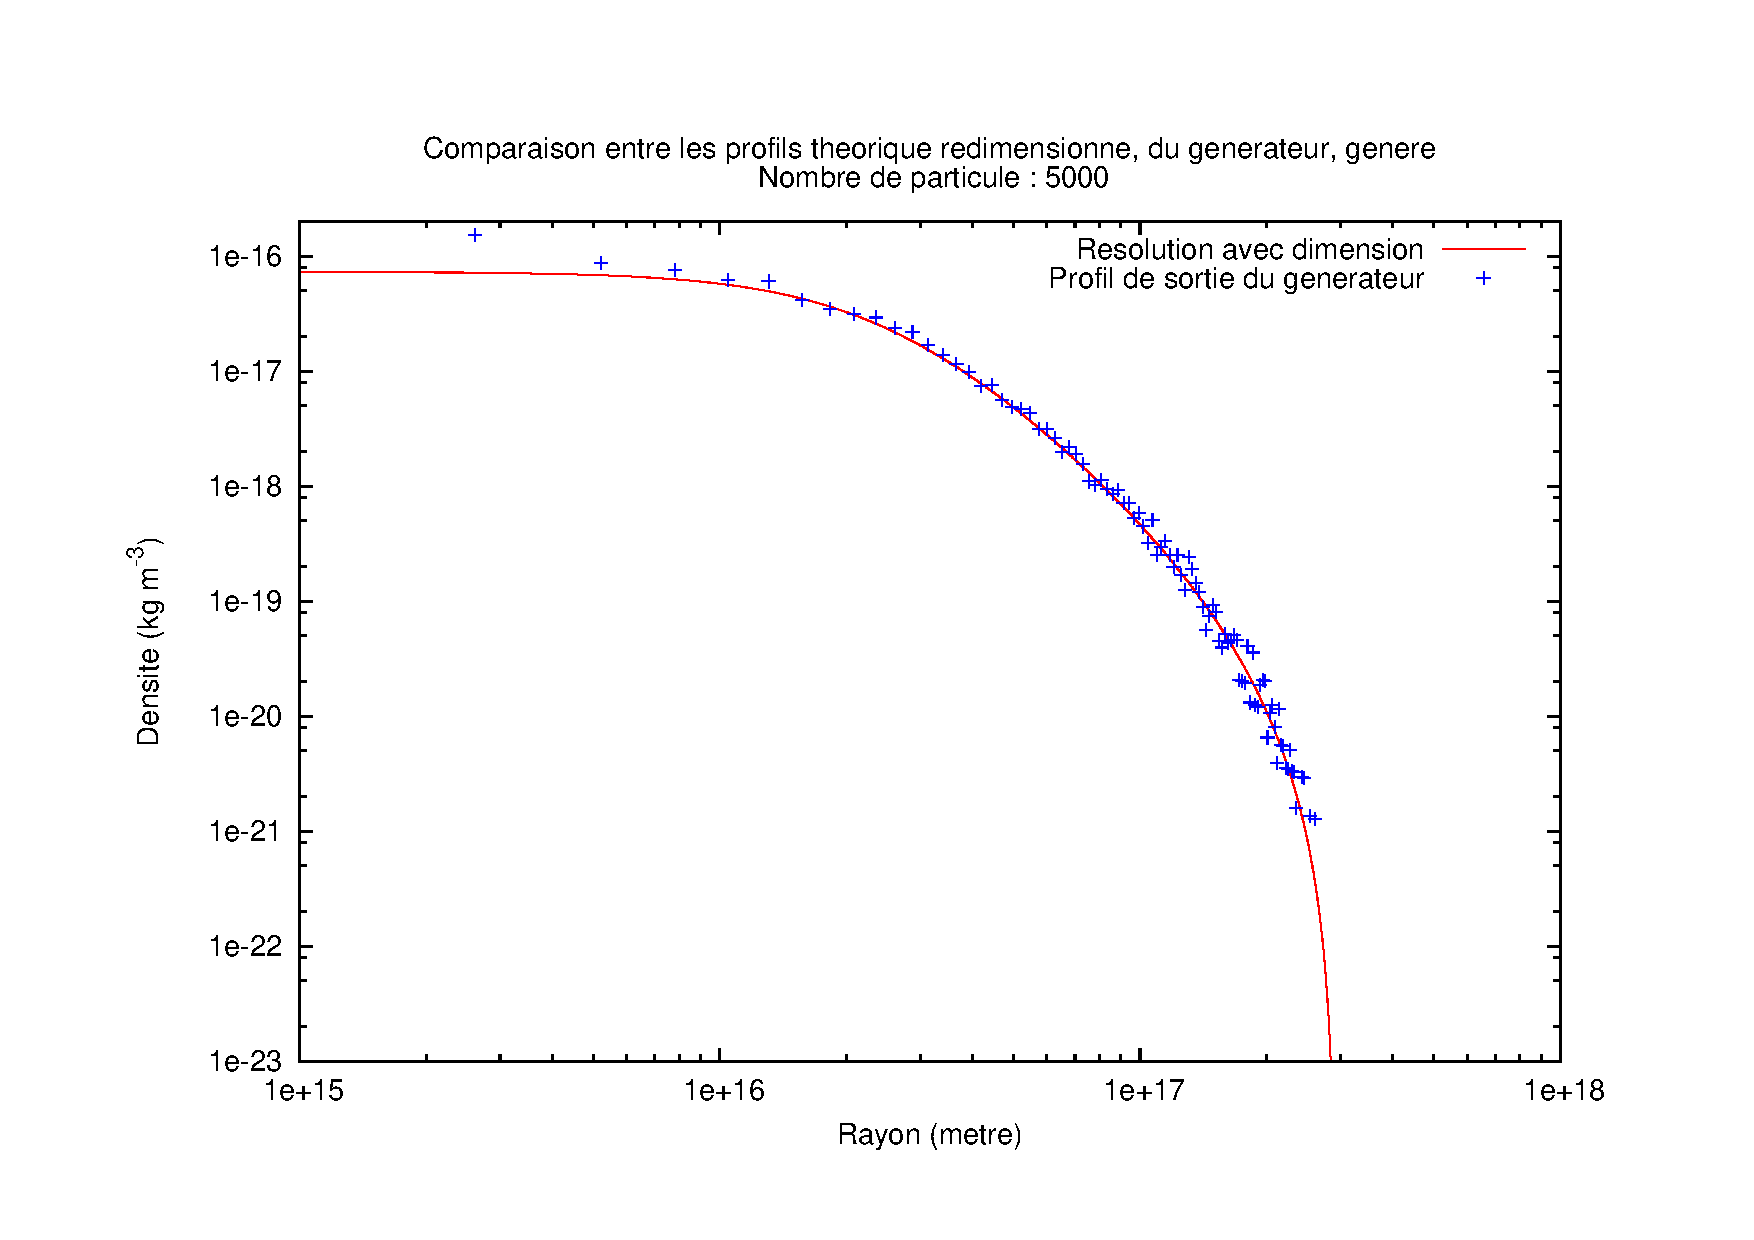
\includegraphics[scale=0.5]{graphe/Comp_dens_gene-theo_5000.pdf}
				% \caption{Comparaison entre la résolution numérique et la densité donnée par le générateur\label{Comp_gene-theo}}
			% \end{figure}
			\begin{figure}[h!]
				% \centering 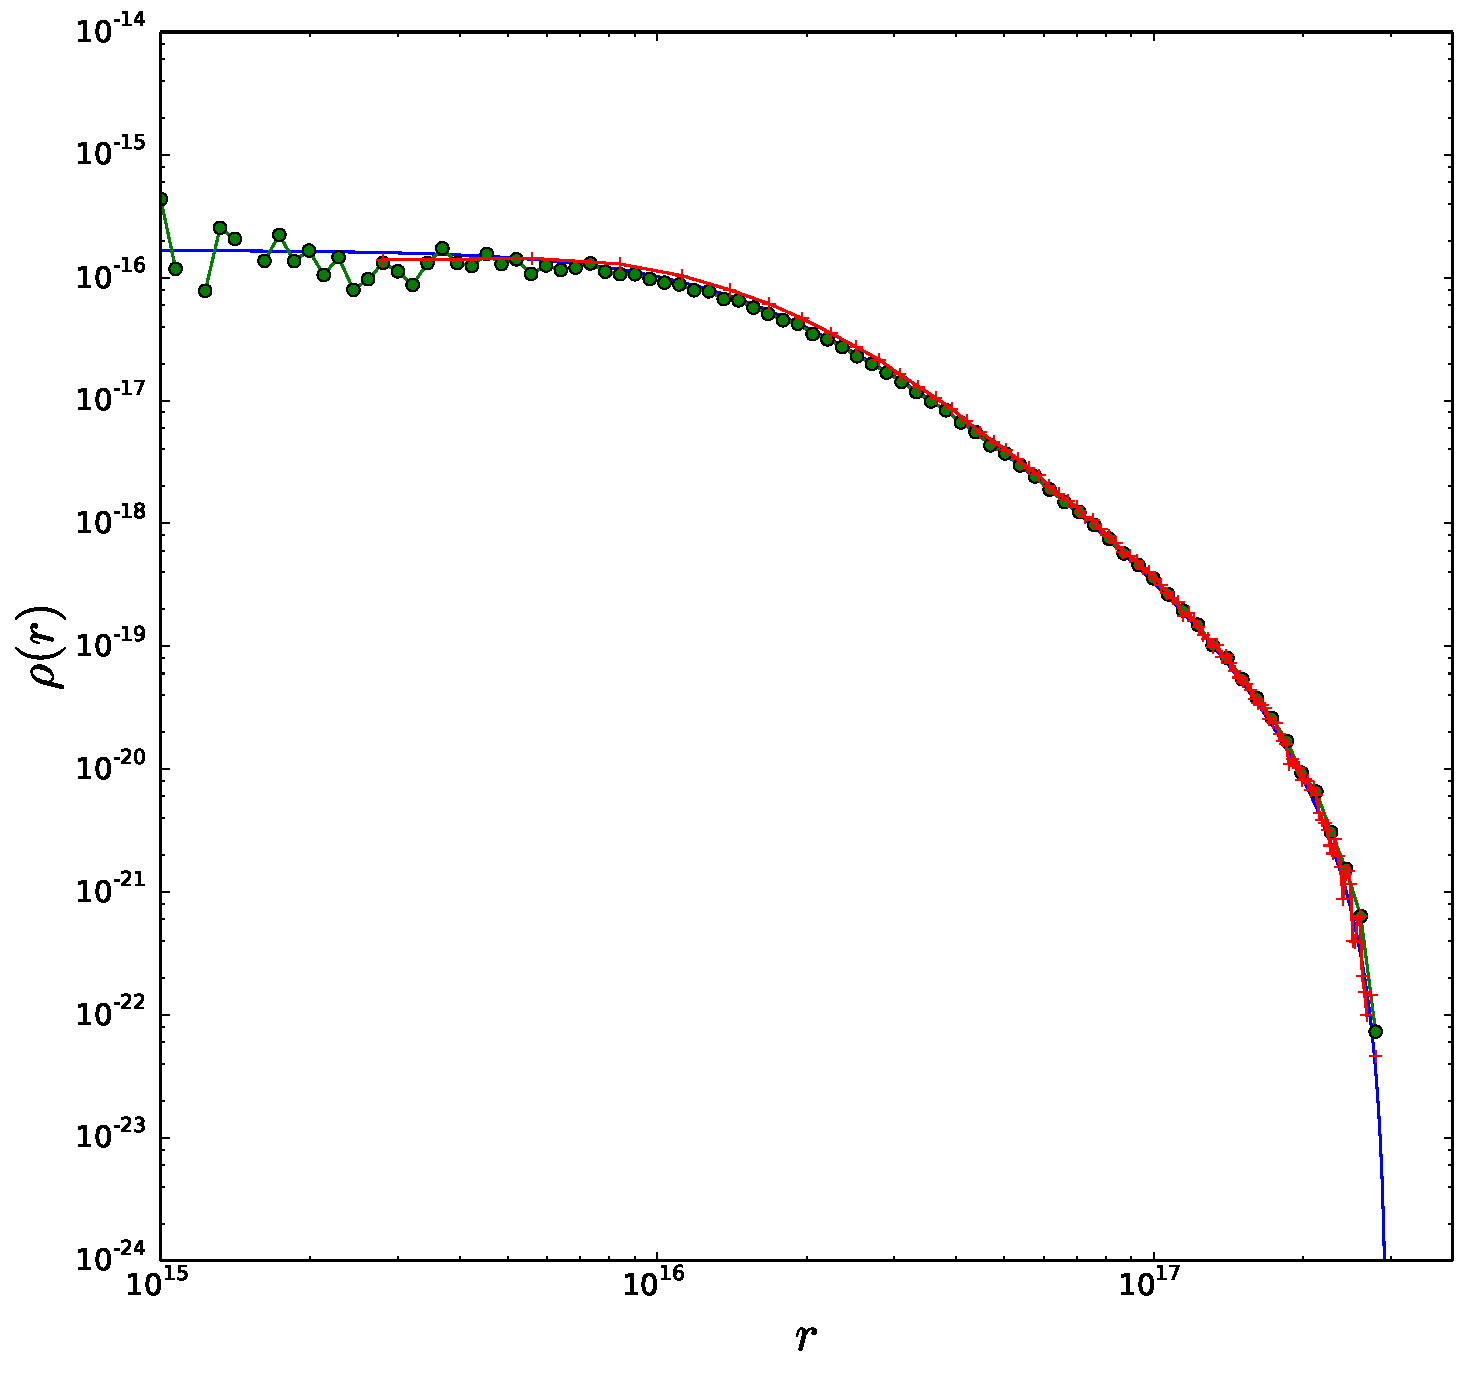
\includegraphics[scale=0.5]{king_model_verification}
				% \centering 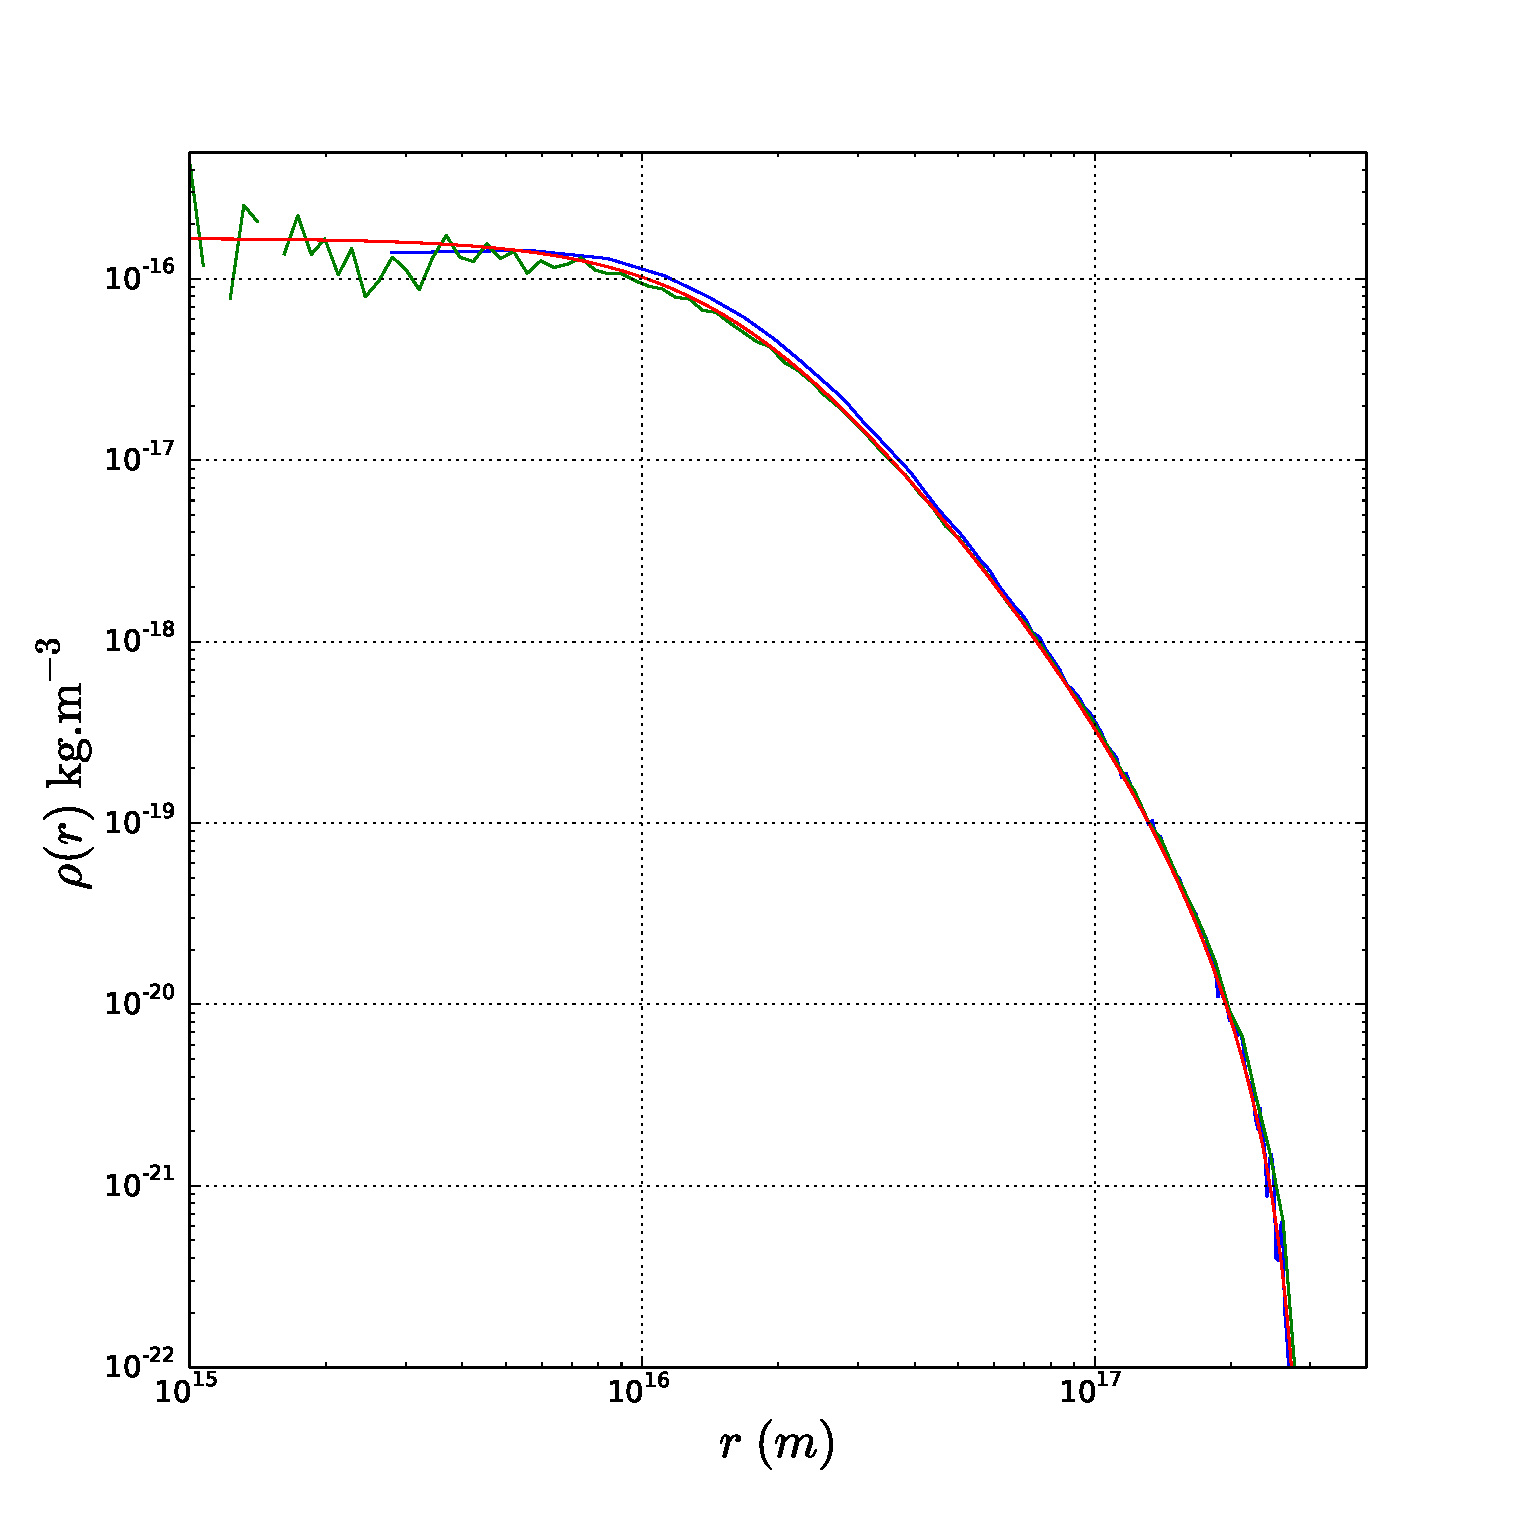
\includegraphics[scale=0.3]{verif_densite.pdf}
				\centering 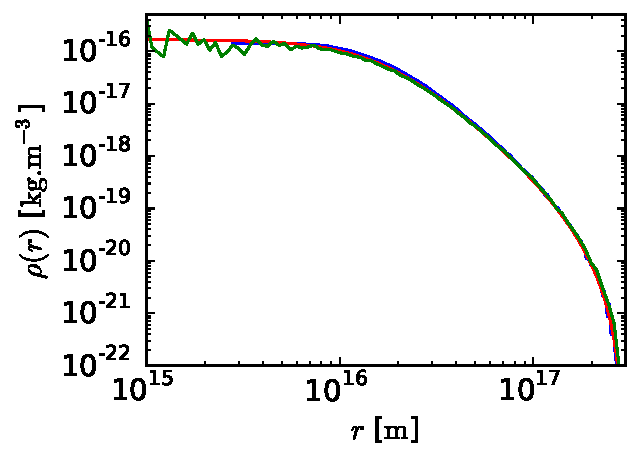
\includegraphics{verif_densite_new.pdf}
				\caption{Comparaison entre la résolution numérique et la densité donnée par le
				générateur\label{Comp_gene-theo}. La courbe rouge correspond à la densité théorique, la
				courbe verte à la densité utilisant les intervalles espacés logarithmiquement et la courbe bleue
				à la méthode décrite ici.}
			\end{figure}

		\subsection{Énergie et potentiel}

			La partie la plus complexe de l'obtention des observables est le calcul de l'énergie. Deux
			choix s'offrent à nous:
			\begin{itemize}
				\item la méthode force brute dans laquelle nous calculons l'énergie totale en utilisant
					l'expression newtonienne du potentiel:
					$$
						E_{tot} = \frac{1}{2}\sum_{i = 1}^{N} m_i v_i^2 - G \sum_{i = 1}^{N} \sum_{j < i}^N \dfrac{m_i m_j}{||r_i - r_j|| + \epsilon}
					$$
					avec $N$ le nombre de particule. Le problème de cette méthode est qu'elle nécessite $N^2$
					opérations et n'est donc pas opérationnelle lorsque nous travaillons avec un grand
					nombre de particules.

				\item la méthode utilisant l'octree décrit précédemment.
		\end{itemize}
		% C'est cette dernière méthode que nous avons utilisée. Nous allons parcourir l'arbre comme décrit dans la
		% section~\ref{Sec::KdTree}. Lorsque nous arrivons sur une feuille, nous calculons les interactions de chaque
		% particules avec celle dont nous voulons le potentiel. Lorsqu'un cube possède un diamètre angulaire trop
		% faible, les particules qu'il contient sont ramenées à une macro particules ayant pour position leur centre
		% de masse et comme masse la masse totale des particules du cube.
		La figure~\ref{potentiel_5000} montre le
		potentiel théorique superposé au modèle de King décrit plus haut.

		En plus du potentiel, nous en profitons pour calculer l'énergie cinétique pour obtenir finalement
		l'énergie totale du système et le rapport du Viriel $\gamma = \frac{2E_c}{E_p}$.

		% c'est le centre de masse des particules qu'il  conti

			% \begin{itemize}
				% \item la méthode force brute : nous calculons l'énergie totale en utilisant
					% l'expression newtonienne du potentiel :
					% $$
						% E_{tot} = \frac{1}{2}\sum_{i = 1}^{N} m_i v_i^2 - G \sum_{i = 1}^{N} \sum_{j < i} \dfrac{m_i m_j}{|| r_i - r_j ||}
					% $$
					% avec $N$ le nombre de particule Le problème de cette méthode est qu'elle nécessite $N^2$
				% opérations et n'est donc pas intéressante lorsque nous travaillons avec un grand
				% nombre de particules. De plus, si deux particules sont très proche,
				% l'énergie potentielle va diverger.
				% \item la réflexion : nous avons déjà calculé la densité, et nous avons
					% la fonction de masse, nous avons tout ce qu'il nous faut pour
					% avoir le potentiel à partir de l'équation de \textsc{Poisson}.
			% \end{itemize}

			% Nous allons calculer le potentiel en résolvant l'équation de \textsc{Poisson}. Voyons
			% comment la résoudre avec ce que nous avons.
			% \begin{align}
				% \Delta\psi &= \frac{1}{r^2}\dfrac{d}{dr}\( r^2 \dfrac{d \psi(r)}{dr} \) = 4\pi G \rho(r) \notag \\
				% r^2 \dfrac{d \psi(r)}{dr} &= 4\pi G \int_0^r \rho(r) r^2 dr = G M(r) \notag \\
				% \intertext{La densité est une fonction continue par morceau, nous pouvons donc écrire :}
				% M(r)    &= 4\pi \int_0^r \rho(r) r^2 dr \notag \\
					% &= 4\pi \sum_{j = 0}^{i - 1} \int_{j \mathrm{dr}}^{(j+1)\mathrm{dr}} \rho_j r^2 dr + 4\pi \int_{r_{i-1}}^r r^2 dr \text{, $r\in\left[ r_{i - 1}; r_i \right]$} \notag \\
					% &= 4\pi \sum_{j = 0}^{i - 1} \rho_j \left[ \dfrac{r^3}{3} \right|_{j \mathrm{dr}}^{(j+1)\mathrm{dr}} + 4\pi\rho_i\left[\dfrac{r^3}{3}\right|_{r_{i - 1}}^{r} \notag \\
					% &= 4\pi \sum_{j = 0}^{i - 1} \dfrac{\rho_j}{3} \mathrm{dr}^3 \( (j+1)^3 - j^3)\) + \dfrac{4\pi \rho_i}{3} \(r^3 - i^3\mathrm{dr}^3\) \notag \\
					% &= M(r_{i-1}) + \dfrac{4\pi \rho_i}{3} \(r^3 - i^3\mathrm{dr}^3\) \notag \\
				% \intertext{Ceci nous permet alors d'écrire le potentiel :}
				% \psi(r) - \psi(0) &= G \int_0^r \dfrac{M(r)}{r^2} dr \notag \\
				% \psi\(r_i\) - \psi(0) &= G \sum_{j = 0}^{i} \left\{\int_{j \mathrm{dr}}^{(j+1)\mathrm{dr}} \dfrac{M(r_{j-1})}{r^2} + \dfrac{4\pi \rho_j}{3 r^2} \(r^3 - j^3\mathrm{dr}^3\) dr\right\} \notag \\
				% \intertext{avec $ r_i = (i+1) \mathrm{dr} $}
				% \psi(r_i) - \psi(0) &= G \sum_{j = 0}^{i} \left\{M_{j-1} \left[ \dfrac{-1}{r}\right|_{j \mathrm{dr}}^{(j+1)\mathrm{dr}} + \dfrac{4\pi \rho_j}{3} \( \left[ \dfrac{r^2}{2} \right|_{j \mathrm{dr}}^{(j+1)\mathrm{dr}} - j^3\mathrm{dr}^3 \left[ \dfrac{-1}{r}\right|_{j \mathrm{dr}}^{(j+1)\mathrm{dr}} \)\right\} \notag \\
						    % &=  G \sum_{j = 0}^{i} \left\{\dfrac{1}{j ( j + 1 ) \mathrm{dr}} \( M_{j - 1} - \dfrac{4\pi \rho_j}{3}j^3\mathrm{dr}^3 \) + \dfrac{4\pi \rho_j}{6}\( 2 j + 1 \)\mathrm{dr}^2\right\}
				% \intertext{Pour le bin central $j = 0$, nous avons :}
				% \psi(dr) - \psi(0)  &=  G \dfrac{4\pi \rho_0}{6}\mathrm{dr}^2
			% \end{align}

			% Pour obtenir la constante $\psi(0)$, nous allons nous servir des conditions sur le bord du système. En effet, nous avons vu plus haut que :
			% \begin{align}
				% \psi_\mathrm{max} = \psi(R) &= - \frac{G M}{R} \\
				% \intertext{Donc :}
				% \psi(R) + \psi(0) - \psi(0) &= - \frac{G M}{R} \\
				% \psi(0) &= - \frac{G M}{R} - \(\psi(R) - \psi(0)\) \\
				% \psi(0) &= \frac{E_l}{m} - \(\psi(R) - \psi(0)\)
			% \end{align}

			% Le graphique~\ref{potentiel_5000} nous montre le potentiel théorique et le potentiel calculé par cette méthode.

			\begin{figure}[h!]
				% \centering 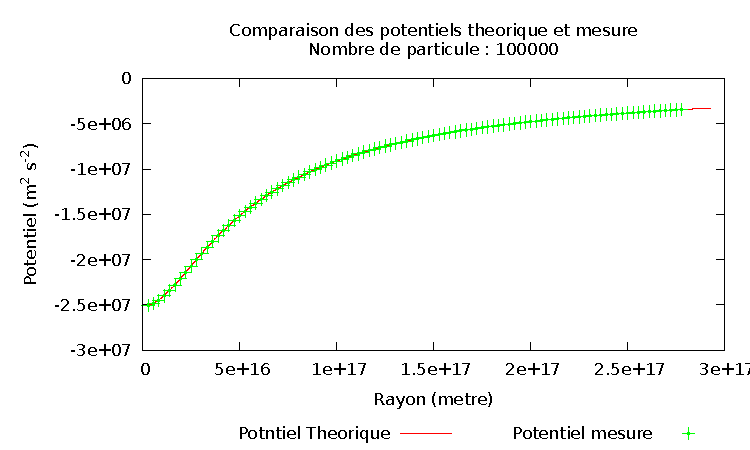
\includegraphics{graphe/Potentiel_ci-100000.pdf}
				% \centering 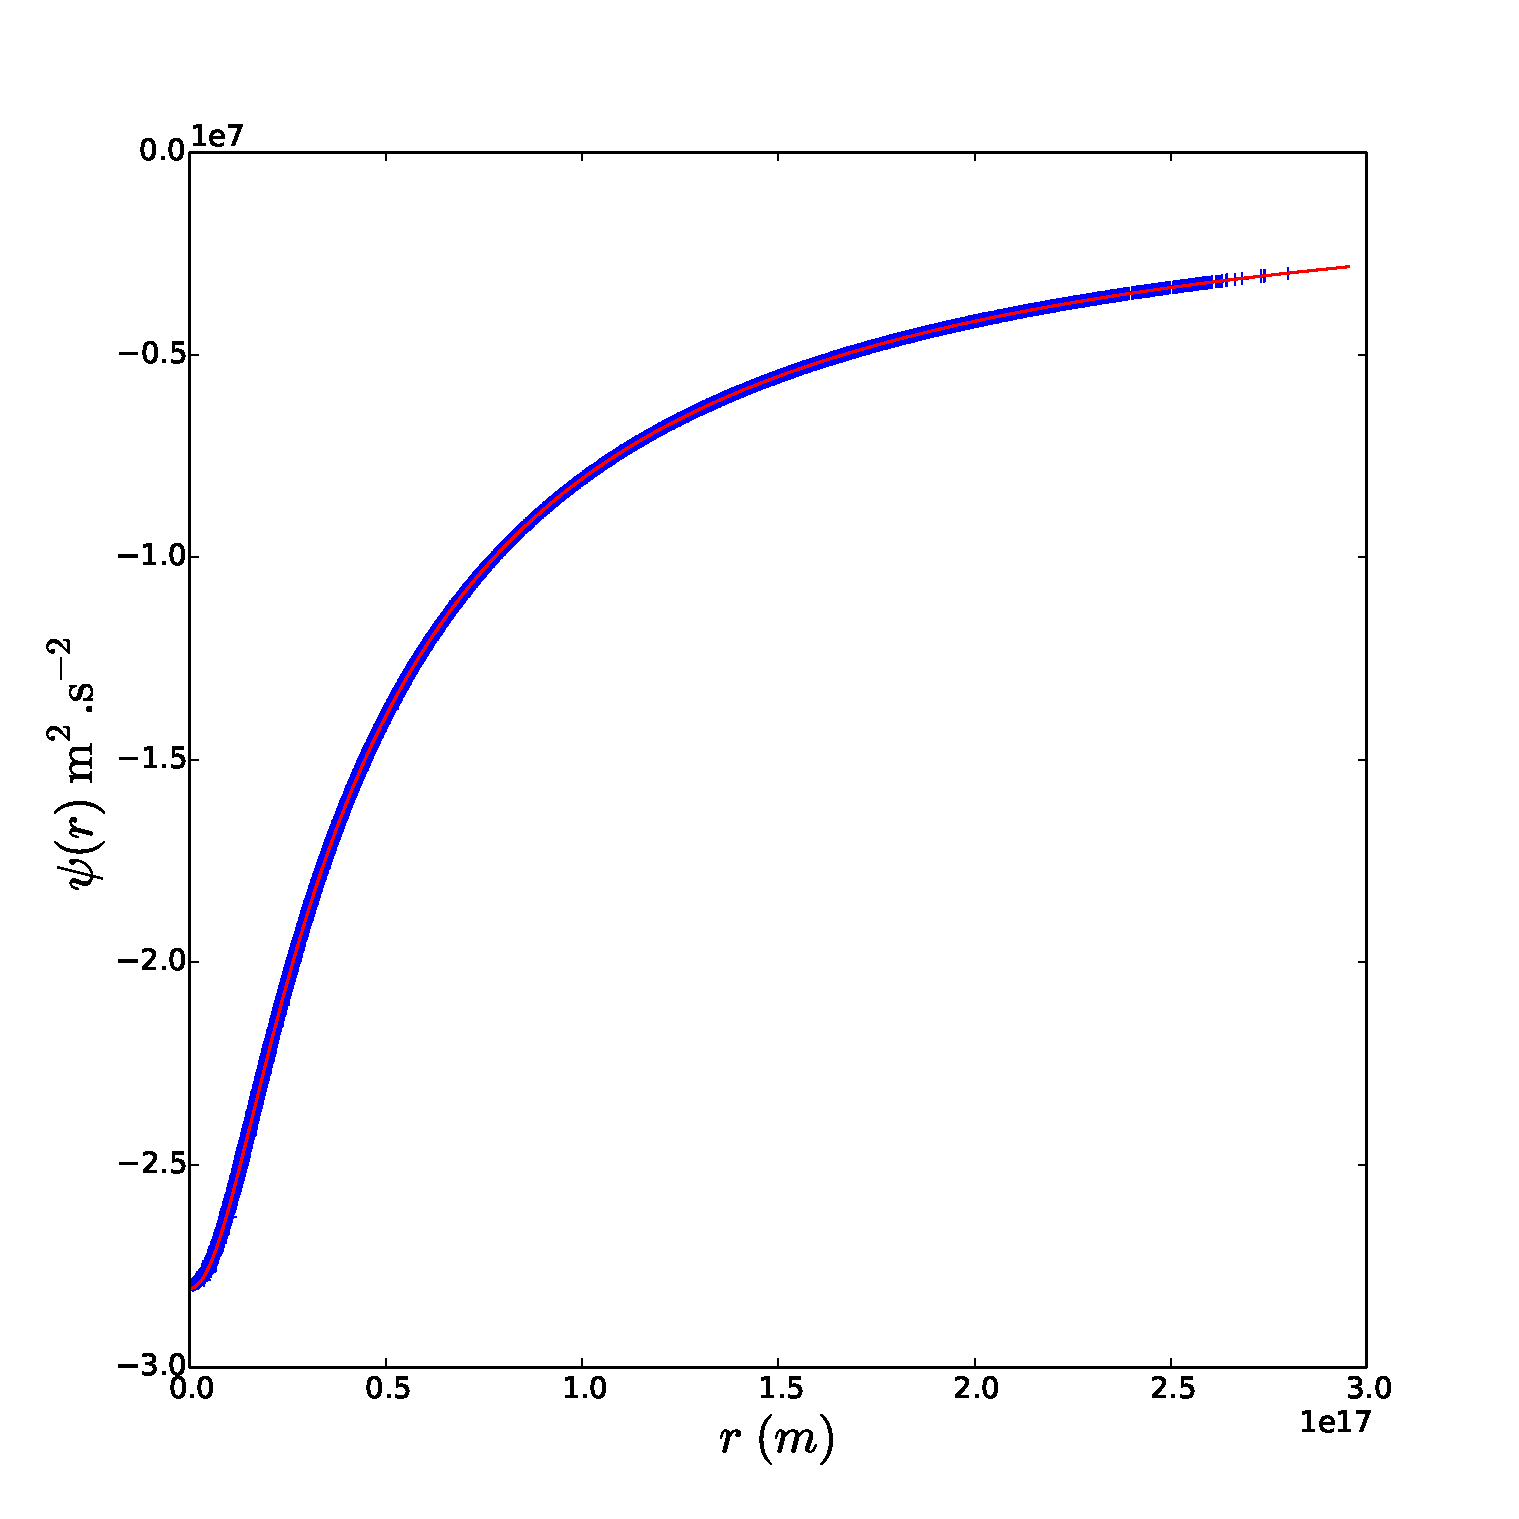
\includegraphics[scale=0.4]{verif_potentiel.pdf}
				\centering 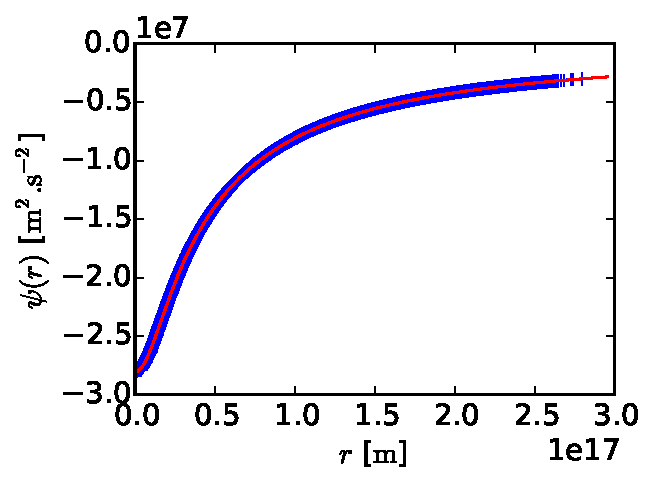
\includegraphics{verif_potentiel_new.pdf}
				\caption{Comparaison entre le potentiel théorique (courbe rouge) et le potentiel donné par le
					générateur (courbe bleu)\label{potentiel_5000}.}
			\end{figure}

		\subsection{Anisotropie des vitesses et forme de l'amas}

			Nos conditions initiales correspondront généralement à des systèmes sphériques et isotropes en vitesse, mais
			qu'en est-il de l'état final?
			Afin de suivre l'évolution de la forme et de l'anisotropie des vitesses de nos systèmes au cours
			du temps, nous avons développé deux observables:
			% Pour savoir si les systèmes sont resté dans ces conditions ou ont
			% vu leurs forme ou distribution de vitesse changer, nous calculons en plus deux autres quantités:
			l'indicateur d'anisotropie et les rapport d'axe de la matrice d'inertie.

			L'indicateur d'anisotropie des vitesses est défini comme suit:
			\begin{align}
				\beta(r) = 1 - \dfrac{\sigma_t^2(r)}{2\sigma_r^2(r)}
			\end{align}
			avec $\sigma_t$ la dispersion de vitesse tangentielle et $\sigma_r$ la dispersion de vitesse
			radiale. Pour obtenir ces dispersions, nous calculons, pour chacune des coquilles de la
			figure~\ref{schema::bin}, les vitesses tangentielles moyennes et les vitesses radiales moyennes,
			puis les dispersions de vitesses correspondantes.
			Lorsque $\beta(r) \equiv 0$, le système est isotrope, pour $\beta(r) \rightarrow 1$ le système
			est radial en vitesse et enfin quand $\beta(r) < 0$ le système est tangentiel.
			Cet indicateur va nous permettre de déceler l'apparition d'une éventuelle instabilité
			d'orbite radiale.

			% Le dernier point à vérifier est la conservation de la sphéricité de nos systèmes. En effet, sauf
			% dans le cas de conditions particulière, comme une instabilité d'orbite radiale, la forme
			% sphérique doit être conservée au cours de l'évolution, voir~\citet{JPerez96}.
			% Maintenant que la densité et le potentiel de l'amas
			% généré ont été vérifiés, il faut aussi vérifier que
			% l'amas ne change pas de forme : nous générons un amas
			% sphérique, nous devons~\footnote{il a en effet été
			% montré qu'un \textsc{King} non collisionnel est
			% stable~\citet{JPerez96}} conserver un amas sphérique
			% après l'avoir fait évoluer.
			% Pour vérifier que la forme
			% de l'amas ne change pas, nous allons regarder comment
			% évoluent les axes principaux d'inertie. Pour ce faire,
			% nous allons calculer les valeurs propres \mbox{$\lambda_1 > \lambda_2 > \lambda_3$} de la matrice
			% d'inertie:
			Pour surveiller l'évolution de la forme du système, nous calculons les valeurs propres
			\mbox{$\lambda_1 > \lambda_2 > \lambda_3$} de la
			matrice d'inertie:
			\begin{align*}
				% \mathfrak{I} &= \(\begin{array}{ccc}
							% \int \(y^2 + z^2\) dm & - \int xy dm & - \int xz dm \\
							% -\int xy dm & \int \(x^2 + z^2\) dm & - \int yz dm \\
							% -\int xz dm & -\int yz dm & \int \(x^2 + y^2\) dm
						% \end{array}\) \\
				% \intertext{avec $dm$ l'élément de masse.}
				\mathfrak{I}   = \(\begin{array}{ccc}
							A & - D & - E \\
							-D & B & - F \\
							-E & -F & C
						\end{array}\)
				% \intertext{L'équation aux valeurs propres va alors s'écrire :}
				% \left|\mathfrak{I} - \lambda \mathbb{I}\right|  &= \(A - \lambda\)\left[\(B-\lambda\)\( C-\lambda\) - F^2\right] + D \(-D\(C-\lambda\) - F E\) - E \left[ D F + E\(B - \lambda\)\right] \notag
				\intertext{Toutes les particules ayant la même masse, il suffira de prendre:}
				\begin{array}{cc}
					\displaystyle A = \sum_{i= 1}^N y_i^2 + z_i^2  &
					\displaystyle D = \sum_{i= 1}^N x_iy_i  \\
					\displaystyle B = \sum_{i= 1}^N x_i^2 + z_i^2  &
					\displaystyle E = \sum_{i= 1}^N x_iz_i  \\
					\displaystyle C = \sum_{i= 1}^N y_i^2 + x_i^2  &
					\displaystyle F = \sum_{i= 1}^N y_iz_i  \\
				\end{array}
			\end{align*}
			où $x_i$, $y_i$, $z_i$ sont les coordonnées de chaque particules du système.
			% polynôme d'ordre 3 que l'on résout avec la méthode de \textsc{Cardan}.

			Une fois ces valeurs propres obtenues, nous traçons l'évolution des rapports d'axe (\og axial ratio\fg)
			$a_1 = \lambda_1 / \lambda_2$ et $a_2 = \lambda_3 / \lambda_2$. Quand $a_1 = a_2 = 1$, le
			système est sphérique. Si $a_2 < 1$ et $a_1 = 1$, le système présente une forme allongée
			caractéristique de l'instabilité d'orbite radiale; et enfin, pour $a_1 >
			1$ et $a_2 < 1$ le système est triaxial. Cette observable va donc nous être très utile pour
			détecter l'apparition d'instabilités morphologiques comme l'instabilité d'orbite radiale.
			% les
			% valeurs propres étant numérotées dans l'ordre
			% décroissant .

			Nous récupérons aussi les rayons à $10\%$ ($R_{10}$), $50\%$ ($R_{50}$) et à $90\%$ ($R_{90}$) de masse qui vont nous
			permettre de suivre l'évolution de la structure du système.

		\subsection{Température cinétique}

			La dernière observable que nous souhaitons obtenir est la température. La température que nous
			calculons est la version discrète de celle donnée dans le chapitre~\ref{King::Chapitre}:
			\begin{align}
				T(r) &= \dfrac{\displaystyle\int_{-\infty}^{\infty}v^2 f(\vec{x}, \vec{p})\vdp}{\displaystyle\int_{-\infty}^{\infty}f(\vec{x}, \vec{p})\vdp} \\
				     &= \dfrac{1}{N-1}\sum_{i=0}^N (v_i - <v>)^2
				     % &= \dfrac{\displaystyle\int_{-\infty}^{\infty}4\pi v^4 f(\vec{x}, \vec{p})\dx{v}}{\rho(r)} \\
				% T(r) &\simeq \dfrac{\displaystyle\sum_i 4\pi v_i^4 f(r, v_i)}{\displaystyle\sum_i 4\pi v_i^2 f(r, v_i)} \\
				     % &= \dfrac{\displaystyle\sum_i v_i^2 \rho(r)}{\rho(r_i)}
			\end{align}
			où $<v>$ est la vitesse moyenne.
			Cette observable va nous permettre de savoir si les sphères sont chauffées ou refroidies par leurs
			interactions avec un bain thermique, et à quelle rythme.

			\begin{figure}[h]
				\centering 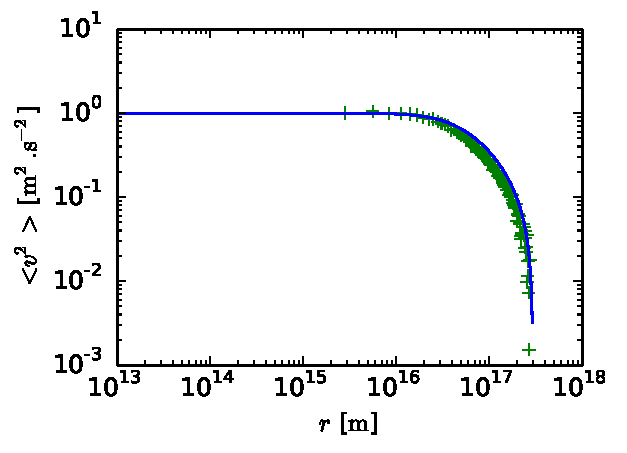
\includegraphics{verif_dispersion.pdf}
				\caption{toto}
			\end{figure}

